\documentclass[a4paper,10pt]{article}
%\documentclass[a4paper,10pt]{scrartcl}

\usepackage{polski}
\usepackage[utf8]{inputenc}
\usepackage{array}
\usepackage{graphicx,footmisc}

%custom margins
\usepackage[left=3cm, top=2.5cm, bottom=3cm, right=2cm, foot=2cm, head=0.5cm]{geometry}
\usepackage{fancyhdr}
\usepackage{longtable}

\title{}
\author{}
\date{}

\pdfinfo{%
  /Title    (Tomasz Boiński)
  /Author   ()
  /Creator  ()
  /Producer ()
  /Subject  ()
  /Keywords ()
}

\begin{document}
\maketitle

\section*{SOVA Symbols}

\begin{longtable}{|c|p{7cm}|} \hline
Name & Graphical representation \\ \hline

Thing &
 \scalebox{0.30}{\includegraphics{./img/thing.png}}
 % class.png: 194x86 pixel, 90dpi, 5.48x2.43 cm, bb=0 0 155 69
 \\ \hline

Nothing &
 \scalebox{0.30}{\includegraphics{./img/nothing.png}}
 % class.png: 194x86 pixel, 90dpi, 5.48x2.43 cm, bb=0 0 155 69
 \\ \hline

Class &
 \scalebox{0.30}{\includegraphics{./img/class.png}}
 % class.png: 194x86 pixel, 90dpi, 5.48x2.43 cm, bb=0 0 155 69
 \\ \hline

Individual &
 \scalebox{0.30}{\includegraphics{./img/individual.png}}
 % class.png: 194x86 pixel, 90dpi, 5.48x2.43 cm, bb=0 0 155 69
 \\ \hline

Property &
 \scalebox{0.30}{\includegraphics{./img/property.png}}
 % class.png: 194x86 pixel, 90dpi, 5.48x2.43 cm, bb=0 0 155 69
 \\ \hline

Datatype &
 \scalebox{0.30}{\includegraphics{./img/datatype.png}}
 % class.png: 194x86 pixel, 90dpi, 5.48x2.43 cm, bb=0 0 155 69
 \\ \hline

Anonymous Class &
 \scalebox{0.30}{\includegraphics{./img/anonymousClass.png}}
 % class.png: 194x86 pixel, 90dpi, 5.48x2.43 cm, bb=0 0 155 69
 \\ \hline

Subclass &
 \scalebox{0.30}{\includegraphics{./img/subclass.png}}
 % class.png: 194x86 pixel, 90dpi, 5.48x2.43 cm, bb=0 0 155 69
 \\ \hline

instanceOf &
 \scalebox{0.30}{\includegraphics{./img/instanceOf.png}} \newline
 \scalebox{0.30}{\includegraphics{./img/instanceOfDatatype.png}}
 % class.png: 194x86 pixel, 90dpi, 5.48x2.43 cm, bb=0 0 155 69
 \\ \hline

equivalentClass &
 \scalebox{0.30}{\includegraphics{./img/equivalentClass.png}}
 % class.png: 194x86 pixel, 90dpi, 5.48x2.43 cm, bb=0 0 155 69
 \\ \hline

disjointWith &
 \scalebox{0.30}{\includegraphics{./img/disjointWith.png}}
 % class.png: 194x86 pixel, 90dpi, 5.48x2.43 cm, bb=0 0 155 69
 \\ \hline

differentFrom / allDifferent &
 \scalebox{0.30}{\includegraphics{./img/allDifferent.png}}
 % class.png: 194x86 pixel, 90dpi, 5.48x2.43 cm, bb=0 0 155 69
 \\ \hline

sameAs &
 \scalebox{0.30}{\includegraphics{./img/sameAs.png}}
 % class.png: 194x86 pixel, 90dpi, 5.48x2.43 cm, bb=0 0 155 69
 \\ \hline

oneOf &
 \scalebox{0.30}{\includegraphics{./img/oneOf.png}}
 % class.png: 194x86 pixel, 90dpi, 5.48x2.43 cm, bb=0 0 155 69
 \\ \hline

unionOf &
 \scalebox{0.30}{\includegraphics{./img/unionOf.png}}
 % class.png: 194x86 pixel, 90dpi, 5.48x2.43 cm, bb=0 0 155 69
 \\ \hline

intersectionOf &
 \scalebox{0.30}{\includegraphics{./img/intersectionOf.png}}
 % class.png: 194x86 pixel, 90dpi, 5.48x2.43 cm, bb=0 0 155 69
 \\ \hline

complementOf &
 \scalebox{0.30}{\includegraphics{./img/complementOf.png}}
 % class.png: 194x86 pixel, 90dpi, 5.48x2.43 cm, bb=0 0 155 69
 \\ \hline

subProperty &
 \scalebox{0.30}{\includegraphics{./img/subProperty.png}}
 % class.png: 194x86 pixel, 90dpi, 5.48x2.43 cm, bb=0 0 155 69
 \\ \hline

inverseOf (property) &
 \scalebox{0.30}{\includegraphics{./img/inverseOf.png}} \newline
\scalebox{0.30}{\includegraphics{./img/inverseOfProperty.png}}
 % class.png: 194x86 pixel, 90dpi, 5.48x2.43 cm, bb=0 0 155 69
 \\ \hline

equivalentProperty &
 \scalebox{0.30}{\includegraphics{./img/equivalentProperty.png}}
 % class.png: 194x86 pixel, 90dpi, 5.48x2.43 cm, bb=0 0 155 69
 \\ \hline

functionalProperty &
 \scalebox{0.30}{\includegraphics{./img/functionalProperty.png}}
 % class.png: 194x86 pixel, 90dpi, 5.48x2.43 cm, bb=0 0 155 69
 \\ \hline

inverseFunctionalProperty &
 \scalebox{0.30}{\includegraphics{./img/inverseFunctionalProperty.png}}
 % class.png: 194x86 pixel, 90dpi, 5.48x2.43 cm, bb=0 0 155 69
 \\ \hline

symmetricProperty &
 \scalebox{0.30}{\includegraphics{./img/symmetricProperty.png}}
 % class.png: 194x86 pixel, 90dpi, 5.48x2.43 cm, bb=0 0 155 69
 \\ \hline

transitiveProperty &
 \scalebox{0.30}{\includegraphics{./img/transitiveProperty.png}}
 % class.png: 194x86 pixel, 90dpi, 5.48x2.43 cm, bb=0 0 155 69
 \\ \hline

hasProperty &
 \scalebox{0.25}{\includegraphics{./img/hasProperty3.png}} 
 %\newline
%\scalebox{0.25}{\includegraphics{elementyGraficzne/hasProperty2.png}}
 % class.png: 194x86 pixel, 90dpi, 5.48x2.43 cm, bb=0 0 155 69
 \\ \hline

domain &
 \scalebox{0.25}{\includegraphics{./img/domain.png}}
 % class.png: 194x86 pixel, 90dpi, 5.48x2.43 cm, bb=0 0 155 69
 \\ \hline

range &
 \scalebox{0.25}{\includegraphics{./img/range.png}}
 % class.png: 194x86 pixel, 90dpi, 5.48x2.43 cm, bb=0 0 155 69
 \\ \hline

allValuesFrom &
 \scalebox{0.25}{\includegraphics{./img/allValuesFrom.png}}
 % class.png: 194x86 pixel, 90dpi, 5.48x2.43 cm, bb=0 0 155 69
 \\ \hline

someValuesFrom &
 \scalebox{0.25}{\includegraphics{./img/someValuesFrom.png}}
 % class.png: 194x86 pixel, 90dpi, 5.48x2.43 cm, bb=0 0 155 69
 \\ \hline

minCardinality / maxCardinality &
 \scalebox{0.30}{\includegraphics{./img/cardinalityminmax.png}}
 % class.png: 194x86 pixel, 90dpi, 5.48x2.43 cm, bb=0 0 155 69
 \\ \hline

cardinality &
 \scalebox{0.30}{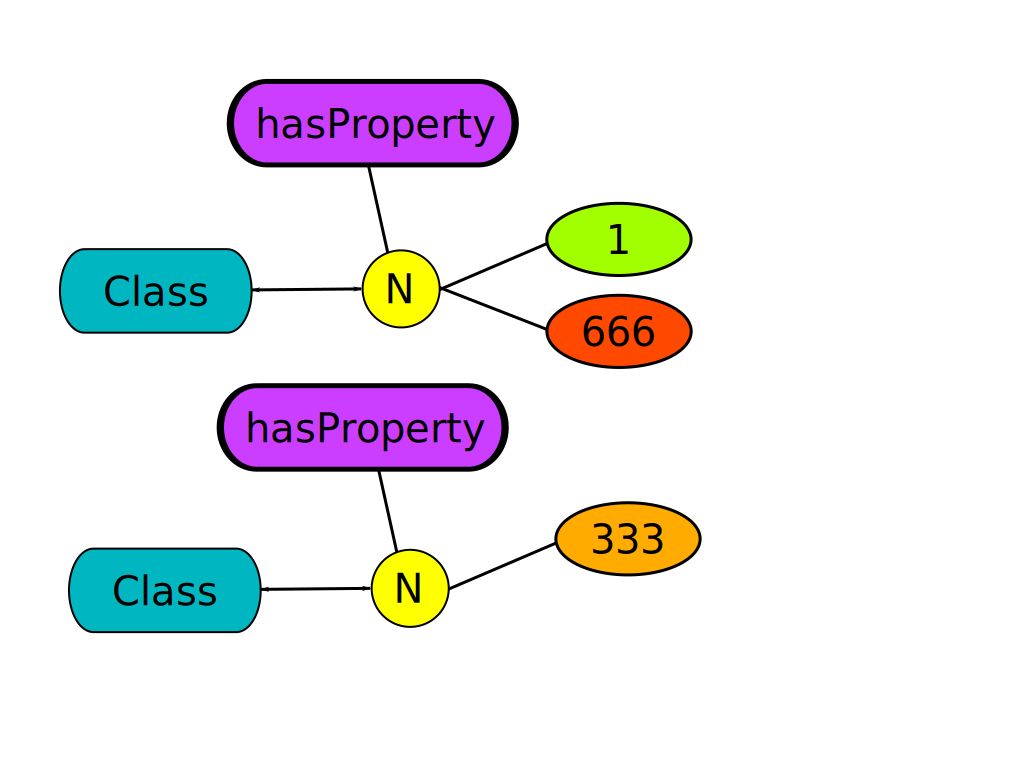
\includegraphics{./img/cardinality.png}}
 % class.png: 194x86 pixel, 90dpi, 5.48x2.43 cm, bb=0 0 155 69
 \\ \hline


\end{longtable}

\end{document}
